% NEED TO WRITE ABOUT HOW THE LABELLER WORKS: THROWS AWAY SMALL SEGMENTS (< 6 FRAMES), MERGES NEARBY SEGMENTS, GENERALLY SMOOTHES DATA
%
% Remember to mention that video quality isn't used after phase 1 due to the side effects cased by labeling the video (namely that bad quality segments don't receive any labels). in a real world application this quality measure could be used to reduce the amount of data to analyze. This should probably be in the discussion section or the summary section for this phase.
%
% Contrast metadata er faktisk aldrig brugt, er det?
%
\chapter{Grouping and labeling}
%
Grouping and labeling comes down to extracting information about what is happening in a piece of video footage. We want to be able to distinguish between different \textit{types} of scenes so we have a way to structure the final video summaries. We want to be able to define a sequence of different scene types that should be put together.
%
\section{Literature Study}
%
There are many ways to extract context from images, sound and video. Some focus on the depicted scene itself, while others look at the events happening in the scene. Location and time of day would be an example of the former while elements such as excitement, violence and other specific behaviour are examples of the later.\\
Hanjalic, A. \cite{citeulike:405480} describes a way to identify regions of high levels of excitement in sports videos based on a manually selected set of features. These features can be both visual (e.g. movement in an image or change of camera position) or audial (based on the energy contained in the audio track).\\
Optical Flow, as described by Bouguet \cite{Bouguet2000}, can also be used to detect events or objects in video. Optical Flow analyses changes in the intensity pattern in images. In many cases this indirectly indicate changes in the 3D scene caused by moving objects or a change of view-point. [REFS] describes ways to identify certain types of actions occuring within videos, such as violent behaviour and [REF] looks at general crowd movement in public places.\\
% Lauge: Der skal skrives lidt mere til disse artikler.
Reisman et. al. \cite{CrowdDetectionInVideoSequences} describes a way to identify crowds of pedestrians from a moving vehicle by detecting inward moving optical flow. I.e. flow which is highly likely to be caused by moving objects and not a change of view-point.\\
Arandjelović \cite{Arandjelovic08crowddetection} attempts to identify crowded regions in still images based on the hypothesis that crowds contain a certain general structure, namely that an image with crowds in it will contain regions, which at a close scale resembles individual people, while at a larger scale will contain repetative structures.\\
% Lauge: Flere crowd detection artikler?
Zhong et. al. \cite{10.1109/CVPR.2004.78} describes a technique for unsupervised detection of unusual events in a video stream. The entire stream is divided into overlapping 4 second segments from which an overall movement pattern is established. Individual segments that differ too much from this patter are considered unusual.\\
% Lauge: Day/Night article her?
% Lauge: Jeg har rykket Haar Cascade classifier ned i sit eget afsnit under Method, men måske skal vi lige have en enkelt linje om det her
Angin et. al \cite{10.1109/MDM.2010.71} describes a method of automatically detecting the color of traffic lights. % Lauge: Vi skal lige have læst/skrevet lidt mere om denne og evt. relation til police blinker detecion
%
\section{Method}
%
The labeling happens in two phases. First we extract different kinds of metadata from the individual videos. This is done frame-by-frame, for each type of metadata, so we end up with a collection of describing properties throughout each video. Some of the metadata is directly available from the earlier phases of the project. The level of \textit{contrast} and the \textit{shift vector magnitudes} described in section \ref{} and revisited below in sections \ref{sec:contrastdata} and \ref{sec:svmdata}, are examples of this. We use the frame mean pixel intentisity to estimate overall brightness (section \ref{sec:brightnessdata}) and seperate the blue color channel (section \ref{sec:blue_channel}). People detection (section \label{sec:peopledata}) is done using Haar cascade classifiers and Optical flow (section \ref{sec:opticalflowdata}) is used for extracting additional event information.\\
\\
The actual labeling is subsequently done by analysing the metadata in a collection of classifiers. Section \ref{sec:police_detection} describes a \textit{police blinker} classifier, which searches for oscillation in the blue channel from the individual frames. Section \ref{sec:overviewclassifier} describes an \textit{overview} classifier, which attempts to detect footage containing litle egomotion (camera movement). In section \ref{sec:verticaloscillationclassifier} we attempt to identify vertical oscillating movement in the optical flow, using it as an indicator for people jumping or signs being lifted into the air. Section \ref{sec:incrowd} describes an \textit{in-crowd} classifier, which uses facial- and person- detection to detect footage with several people in it. In section \label{sec:infocus} we further explore the area of people detection, by looking for footage, which focuses on a specific (assumably interesting) person for a duration of time. Finally, in section \ref{sec:daynightclassifier} we look at differentiating between day- and night- time footage by working with the different brightness and color intensity metadata we have extracted.
%
\subsection{Metadata}
%
This section describes the different type of metadata we extract.
%
\subsubsection{Contrast}\label{sec:contrastdata}
%
The \textit{contrast} in a frame is defined as being the standard deviation of the intensity values in the image-matrix. This is described in detail in section \ref{}. A small deviation would indicate little contrast/diversity in color-intensity, and a large deviation would indicate a high contrast/much diversity in intensity. The \textit{contrast} metadata for each video consist of the set of these standard deviations for each frame.
%
\subsubsection{Shift vector magnitude}\label{sec:svmdata}
%
Like the contrast, the \textit{shift vector magnitudes} for each video is already computed as a part of the initial image quality assessment, as described in section \ref{}. We make a rough estimation of the egomotion (camera movement) by shifting all pairs of neighbouring frames until they more or less alligns up. This shift is expressed as a vector, whos magnitude tells us how much the camera is moving/shaking at each frame point in the video. The \textit{shift vector magnitude} metadata consists of set of these magnitudes throughout the video. It is used in the \textit{overview} classifier described in section \ref{sec:overviewclassifier}
%
\subsubsection{Brightness}\label{sec:brightnessdata}
%
The \textit{brightness} metadata consists of the mean pixel intensity in each frame throughout the video. It is used in the \textit{day/night} classifier described in section \ref{sec:daynightclassifier}.
%
\subsubsection{Blue color channel}\label{sec:blue_channel}
%
This particular type of metadata is extracted from the original videos (before grayscale conversion). Each frame in a video consists of a matrix of pixels in 3 channels; red, green, and blue. We extract the blue channel for the purpose of police blinker detection, described in detail in section \ref{sec:police_detection}, and day/night detection, described in detail in section \ref{sec:daynightclassifier}.
%
\subsubsection{The presence of people}\label{sec:peopledata}
%
%
%
%
% Lauge: Her skal ryddes op og skrives om. Haar cascade classifier tekst fra andre steder er samlet her under sin egen paragraf.
%
%
%
\paragraph{Haar cascade classifier}
%
With the introduction of Haar Cascade Classifiers (HCC) % Anders: Hvad er dette?
by Viola and Jones\cite{viola01}, later improved upon by Lienhart and Maydt\cite{lienhart01} and by Schmidt and Kasinski\cite{schmidt01}\cite{schmidt02}, there exists a very efficient tool for facial detection. The HCC uses a data-structure called an integral image, an algorithm based on AdaBoost % Lauge: Reference
that selects critical visual features, and a method that combines complex classifiers to compute on the most promising object-like regions. Initial results by Viola achives 15 frames per second detection in an 384 by 288 pixel image using, by todays standards, outdated hardware.\\
\\
We use Haar cascade classifiers \cite{viola01}\cite{lienhart01}\cite{schmidt01}\cite{schmidt02} to detect people and faces in individual frames.
%
%
%
\paragraph{Originalt inhold}
Detecting the presence of people will help us determine if footage was recorded from within a crowd, described in detail in section \ref{sec:incrowd}, or if the footage has focus on a specific person, described in detail in section \ref{sec:infocus}, which indicates that this person is of special interest, ex. a speaker.\\
An integral image (aka. summed area table) is a matrix where any point $(x,y$ is the sum of all pixels above and to the left of $(x,y)$ illustrated in Figure \ref{fig:integral_img}. Not only is the computation of this matrix efficient as a function of its nature (it can reuse already computed sums when building the matrix), the sum at any given point can be computed in constant time as it can be done by 4 lookups in the matrix followed by 4 additions and substractions.
%
\begin{figure}[h]
     \centering
     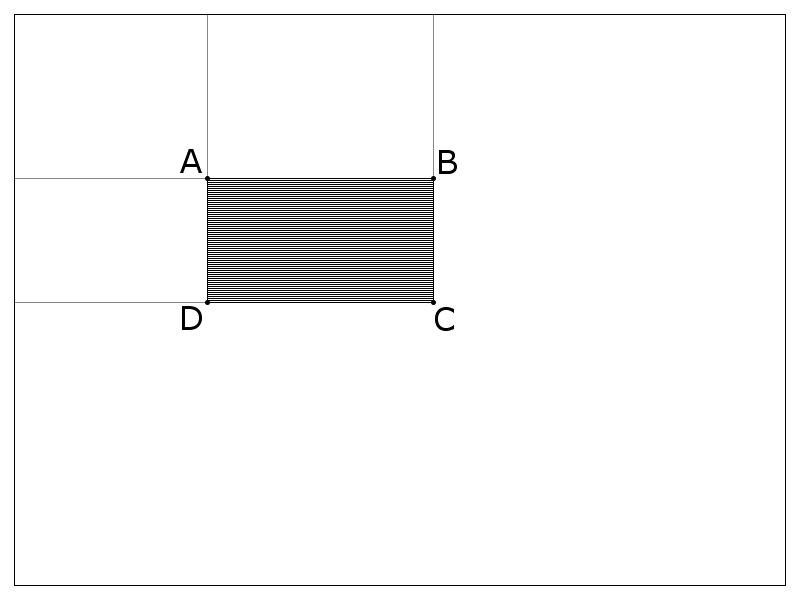
\includegraphics[width=0.75\textwidth]{img/integral_image.png}
     \caption{Integral image}\label{fig:integral_img}
\end{figure}\\
%
AdaBoost (Adaptive Boosting) is a meta-algorithm for boosting machine learning algorithms where subsequent classifiers built are tweaked in favor of those instances misclassified by previous classifiers. The derivative algorithm is a modification of AdaBoost that constrains each returned (weak) classifier to be dependent only on a single feature, which in turn is deemed a critical feature.\\
A method of using less complex processing to detect promising regions, and then apply the more complex processing on these regions.\\\\
%
OpenCV provides a python-implementation of an already trained Haar cascade classifier, manifested as a range of xml-files describing the Haar like features of a human face, both front and profile, aswell as upper body, lower body, and full body.\\
By deploying facial detection to every frame in each video we get a good estimate of how many people are present, and also their location within each frame. This estimate is limited by the quality of the frame, ie. shaky video-clips have a reduced detection rate, and we also experienced a significant increase in false positives for banners and flags (which there is a presence well above normal in our training set).BELONGS IN RESULTS\\
We are working with 480 by 640 pixel images and are able to achieve real-time facial detection (working on video with 24 frames per second). BELONGS IN RESULTS\\
For the sake of simplicity we have not implemented the optimization of only analayzing select frames (ex. every third frame) which we do not believe will have a significant impact on the detection rate as we interpolate the detected objects between frames already.\\
We suggest that further optimizations involve exploiting the ready-at-hand metadata such as the general frame quality which severely impacts facial detection rates in a negative fashion.\\
Further optimization can be achived by exploiting the temporal data. Ie. instead of analyzing the entire frame by expanding the search window incrementally, we utilize knowledge of where people were present in the previous frame. This would require a customized HCC which is a major increase in complexity compared to the other mentioned optimizations.
%
\subsubsection{Optical Flow}\label{sec:opticalflowdata}
%
\paragraph{Optical Flow - Hvordan virker lortet?}
%
For in-frame event extraction we use optical flow \cite{Bouguet2000}.
%
% Lauge: Her skal skrives noget om hvordan optical flow (Lucas Kanade, artiklen ovenfor) fungerer
%
Unfortunately, most of the existing work done on both event- and crowd- classification focuses on settings with stationary cameras. Although Reisman et. al. \cite{CrowdDetectionInVideoSequences} \textit{do} work with images from a camera fixed on a moving vehicle, their appraoch is still not applicable to our scenario, since our videos are recorded mostly by handheld devices, whose movement are a lot less predictable.\\
%
\paragraph{Optical Flow - Hvad gør vi?}
%
Where \textit{shift vector magnitudes} tells us something about how the camera itself moves, optical flow attempts to explain how the content within each frame moves. There has been a substancial amount of research put into this field. Most of our footage is recorded by handheld cameras often under very poor conditions. Extracting the optical flow of our videos is therefore not only a matter of analysing how reference points move around in the frame. First we must estimate the \textit{egomotion} (the motion of the camera) itself, in order to \textit{stabilise} the frame.
%
\paragraph{Frame stabilisation}
%
There are several ways to do this. An option is to use the \textit{shift vector magnitudes} that we have already computed. This intuitively makes sense since they are suppose to describe the movement of the camera at at each frame in the video. However, it turns out that although this data may be suitable for describing the general type of cameara movement (shaking, panning), especially when the data is smoothed across several frames, it has a relatively high margin of error for individual frames. This is especially the case if the camera moves very fast or if there actually \textit{is} a lot of movement within the frame. Another option is use the mean of all the optical flow vectors as the egomotion. Alternatively one could use the most commonly occuring vector. However, our experimentation showed that these two methods suffer from one serious limitation. If moving objects in the frame are very close to the camera, they tend to become more influencial than the stationary background and they end up swapping roles. The egomotion is then based on the movement of the large object, the opposite of what we want. The border-case for this condition is especially problematic. This occurs when a moving object takes up half of the frame. Often, changes in position will then \textit{periodically} cause it to be more or less dominant than the background. In these cases the egomotion vector will jump from one extreme to the other, in close succession, and thus become completely useless.\\
Some of these problems could probably be alleviated through further analysis or averaging across time. However, through our experimentation we came up with an approach that seems more promising.\\
\\
\textit{Corner detection} refers to identifying features in a frame, which are \textit{good to track}. They are areas (or points), which are likely to be clearly distinguishable on the following frames. This is often done by locating areas with low \textit{self simmilarity}. That is, areas that do not look like other areas close by. We found that generally, these points has a tendency to be present in stationary objects in the frame far more often than in moving objects, and thus form a very decent base for our egomotion vector. The implementation we use to identify these features is based on the Shi-Tomasi corner detection algorithm described by Shi et al. \cite{Shi_1994_3266}. We track these features and define our egomotion to be the mean of all the resulting displacement vectors.\\\\
%
Note: We have later come across other, more advanced techniques for calculating the egomotion of a video. Raudies et al. \cite{Raudies:2009:ELM:1612122.1612125} describes such a method. Unfortunately, do to our late discovery of this method we have not been able to test it.
% Lauge: Der skal skrives noget mere om denne metode, hvis den skal nævnes, desuden skal dette rykkes til future work
%
\paragraph{Detecting movement}
%
We now look at the movement within the frames. We do this by placing a grid of points across the frame and perform optical flow analysis on them. We use a pyramidal implementation of the Lucas Kanade feature tracker described by Bouguet \cite{Bouguet2000}.
% Flyt til parameter tuning:
We do the analysis with a grid of 24x16 points, using a search window of 30x30 pixels through two iterations.\\% TODO: ACTUALLY UNDERSTAND THIS and describe it here!!!
%
Some of the resulting vectors are considered invalid if we are unable to track them. This is often the case with points in the sky or in surfaces without any distinct features) or if the point being tracked ends up outside of the subsequent frame. Let $E$ be our egomotion vector. Then, for every vector $v \in V$, where $V$ is the set of valid displacement vectors, the isolated movement vector $v'$ is defined as:
\begin{equation}
v' = v - E
\end{equation}
Let $V'$ describe the set of all isolated movement vectors $v'$. $V'$ then describes the movement of objects within the frames.\\
Each vector $v' \in V'$ describes the movement of one particular point in the original grid. By looking at the different directions of flow we may be able to say something about what is going on in the video. We simplify the data dividing the image up into nine segments as shown in figure [FIGURE REF]. We calculate the mean of the movement vectors in each group, seperately, and use these nine new vectors to describe the overall flow in different parts of the frame.
%
% Lauge: RISK - This model may be too simple, for good results
%
[FIGURE OF BOXES AND GRID]
%
The \textit{optical flow} metadata consist of sets of these nine vectors, calculated for each frame in the video. It is used in the \textit{vertical oscillation} classifier described in secion \ref{sec:verticaloscillationclassifier}.
%
%
%
%
%
\subsection{Label classifiers}
%
Each classifier performs a binary classifaction on a specific label. It analyses all the available footage and returns a collection of indexes to all the segments where it believs the specific label it to be present. These indexes consist of a reference to the video in question, as well as a start and end index. Depending on the classifier, these segments are then post-processed using \textit{segment interpolation} and/or \textit{segment smoothing}
%
\subsubsection{Segment Interpolation}\label{sec:labelmerge}
%
% Lauge: Denne sektion skal skrives om. Den giver ikke meget mening som den er. Desuden skal der skrives noget om 'truncation' som bliver refereret til flere steder senere
%
Segments in a video is easilly fragmented and two segments with the same label just a single frame apart will by all means and purposes be interpreted as such. This is often a result of fragmented metadata, ex. several consequtive frames with people present that our people presence detection algorithm failed to detect. To patch this fault we interpolate the segments by applying the label, $l$, to the frames between segment $a$ and segment $b$ if these are not too far apart (by default 24 frames) and both segments share the same label, $l$. As we are already analyzing segments we also filter out segments of diminutive length, which by default is 5 seconds.
%
\subsubsection{Segment Smoothing}\label{sec:labelsmooth}
%
% Lauge: Denne sektion skal skrives om. Den giver ikke meget mening som den er. Desuden skal der skrives noget om 'truncation' som bliver refereret til flere steder senere
%
If segments are higly fragmented because the label-algorithm that produced them made no attempt to smooth the frames and their respective label (or absence of same) we apply triangle smoothing on the segments, defaulting to a degree of $36$ frames equal to $1.5s$, and subsequently cut off values below a certain treshold, defaulting to $1/3$, ie. values below the treshold are truncated to $0$.
%
\subsubsection{Police Blinker classifier}\label{sec:police_detection}
%
By investigating the blue channel mean of each frame (section \ref{sec:blue_channel}) we are able to detect if the police blinker lights are present in part of a video.% Resultat
We analyze the blue channel mean as a function of time, and if these values are oscillating within certain parameters,% Specific frequency
we have an indication of the precense police blinker lights.
%
\begin{figure}[h]
     \centering
     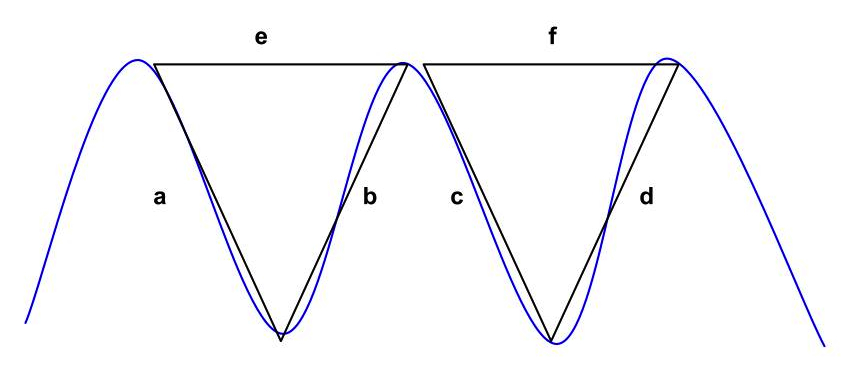
\includegraphics[width=1.05\textwidth]{img/triangles.jpg}
     \caption{}\label{fig:triangles}
\end{figure}\\
% Lauge: Mangler title + Lav rigtig figur
Local minima/maxima in an oscillating graph connected by straight lines will form triangular shapes as illustrated in Figure \ref{fig:triangles}, where consequtive triangles of roughly equal size indicate a steady oscillation. As an alternative to computing the area of each triangle we investigate how the length of the vertices in each triangle deviate from each other
\[
\text{std}([\|a\|,\|b\|,\|c\|,\|d\|]) < \tau_1,
\]
% a,b,c, og d skal defineres i tekst
for some threshold $\tau_1$ where std is the standard deviation. Analogously for the horizontal vertices
\[
\text{std}([\|e\|,\|f\|]) < \tau_2,
\]
% e og f skal defineres i tekst
for some threshold $\tau_2$.\\
The blue channel mean is smoothed using triangle smoothing with a degree of 5% paramter tuning
as this give softer curves on the graph. Oscillating segments are then detected, and nearby segments are merged as described in section \ref{sec:labelmerge} where segments up to 48 frames% paramter tuning
 apart are interpolated into a single segment, and segments shorter than 24 frames% paramter tuning
  are removed.
%
\subsubsection{Person in Focus classifier}\label{sec:infocus}
%
We compute a moving average (over 4 frames ~ 166ms)% paramter tuning
of the people presence metadata but excluding objects detected (partially) outside a centered bounding box.
% Lauge: Det er ikke klart hvad vi prøver at sige her:
A moving average of only 4 frames requires a low frequency of false negatives between frames which in turn makes a greater demand on the quality of each frame (steady or no camera movement, a good shot angle, and little background clutter). The frames and their respective label are smoothed as described in section \ref{sec:labelsmooth} with a smoothness degree of 36,% paramter tuning
equal to $1.5$ seconds, and a truncation value of $1/3$.% paramter tuning
 Nearby segments are merged as described in section \ref{sec:labelmerge} where segments up to 24% paramter tuning
  frames apart are interpolated into a single segment, and segments shorter than 120% paramter tuning
  frames, equal to 5 seconds, are removed.
%
%
\subsubsection{Overview classifier}\label{sec:overviewclassifier}
%
The \textit{overview} classifier attempts to detect footage with negligible egomotion, as well as little internal movement within the frames. Furthermore, in order to avoid overlap with the \textit{person in focus} footage, which often also holds these charactetistics, we also require the overview footage to not focus on any person in particular. The overview classifier uses the \textit{support vector magnitude} metadata described in section \ref{sec:svmdata}, the \textit{optical flow} metadata described in section \ref{sec:opticalflowdata}, as well as the actual labels classified by the \textit{person in focus} classifier described in section \ref{sec:infocus}.\\
We perform a slight triangular smoothing on the metadata in order to remove outliers. We also discard all footage, which has already been classified with the \textit{person in focus} label.\\
% RISK: One label takes precedence over another (not isolated)
We now look at the amount of movement in each part of the image in order to determine if a frame contain too much internal movement. Let the internal movement in a frame be defined as $f_{i} = [m_{1},m_{2} \dots m_{9}]$, where $m_{x}$ is the distance of movement occuring in a specific part the frame, calculated as the mean of the magnitude of all adjusted optical flow vectors, in an area. The number of areas exceeding a given limit, $s$, is then defined as:
%
\begin{equation}
A_{f} = \sum_{i=1}^{9}
\begin{cases}
0 & \text{, if } m_{i} \leq s\\
1 &  \text{, otherwise}
\end{cases}
\end{equation}
%
This way of analysing sub-parts of the image should improve the chance of detecting local charactaristics, which would be lost in an overall analysis of the frame. %Flyt til metadata afsnit?
 Next we combine this meassure with the egomotion in the frame, defined as $f_{e}$. The binary \textit{overview} classification of a frame is defined as:
\begin{equation}
O(f) =
\begin{cases}
0 & \text{, if } A_{f} > t \vee f_{e} > u \\
1 &  \text{, otherwise}
\end{cases},
\end{equation}
where $t$ is a threshold that defines how many areas are allowed to contain too much internal movement, and $u$ is a threshold defining the maximimum \textit{shift vector magnitude} we accept for the frame.
%
\subsubsection{Vertical Oscillation classifier}\label{sec:verticaloscillationclassifier}
%
The \textit{vertical oscillation} classifier attempts to detect footage with vertical movement of objects. Such movement can be caused by people jumping, by people gesticulating heavily whilst talking, or if people are raising signs into the air. In order to do this we look at the variance of the vertical direction of the optical flow vectors over some time.\\
As with the \textit{overview} classifier we analyse the internal movement in different parts of the image, in order to detect local charactaristics. Let the vertical movement in a frame be defined as $f_{v} = [m_{1},m_{2} \dots m_{9}]$, where $m_{x}$ is the vertical movement, calculated as the mean of the vertical movement of the adjusted optical flow vectors, in an area.


we have a set of thresholds, $s$, $t$, and $v$, which are used to regulate the classifier. We start by calculating the standard deviations of the vertical direction of the vectors, throughout the videos. Since the optical flow metadata consists of nine bins of data for each frame, each bin covering one uniuqe ninth of the frame, this is done sepeately for each bin. The parameter $v$ (in our case $v = 12$), determines over how many frames the standard deviation is calculated. Thus, $s$ can be used to determine the frequence of oscillation the classifier should detect. The resulting deviations in each bin are smoothed over 60 frames in order to remove noise, just like in the Overview classifier. We then iterate through all frames and for each of them look in each bin to see if the standard deviation in it is above our threshold, $s$. If this is the case for more than $t$ bins, we consider the frame to contain vertical oscillation.
%
% TODO: Little bit more here...
%
% REMEMBER: Describe RISKS (zooming)
%
%
\subsubsection{In-Crowd classifier}\label{sec:incrowd}
%
% We exploited an inherent limitation in facial detection; that faces far away in the image are rarely detected. Due to the nature of our datasets, and we do not try to cover up in any way that this particular label is highly overfitted for this exact purpose, waranted that when multiple faces,
% %
% % Noter fra Kim: Hvad vil i sige med dette? Pas på blah blah!
% %
% on average 2 or more faces, are detected we would almost certainly be in a crowd or overlooking a crowd from within.\\
% Technically speaking we would compute the moving average over 12 frames (500 ms) of people detected (profile, frontal, or upper body) and if we had detected more than 1 person we would deem that particular frame to be in a crowd.
% %
% % Noter fra Kim: Hvorfor datid?
% %
% One must have in mind that there are 24 frames each second, and the facial detection will far from detect (the same) faces/people in each consequtive frame, even for a fairly still image. Hence we had to interpolate the data to get a good estimate.\\
% This method could be made even more accurate if we instead of employing a moving average would interpolate each bounding box (bounding the detected object), but also a more complex method.
% REWRITE
%
We compute a moving average (over 12 frames/500ms) of the people presence metadata to determine if the frame is shot from within a crowd, or slightly overlooking a crowd. If more than 1 person is present in the frame the frame is deemed to be \textit{in crowd}. Obviously 2 people does not make a crowd, but taking into account the high frequency of false negatives both in and between frames, this shows to provide a good estimate. The frames and their respective label are smoothed as described in section \ref{sec:labelsmooth} with a smoothness degree of 24, equal to 1 second, and a truncation value of $0.9$. Nearby segments are merged as described in section \ref{sec:labelmerge} where segments up to 24 frames apart are interpolated into a single segment, and segments shorter than 60 frames, equal to $2.5$ seconds, are removed.\\
A fallacy in this method are cases of just two people in a frame which are easily detectable, ie. facing a steady camera with no background clutter.\\
An alternative to this method is using optical flow... %LAUGE
%
\subsubsection{Day \& Night classifier}\label{sec:daynightclassifier}
%
Our Day \& Night classifier is mostly a proof-of-concept. The time of creation is stored as part of the video file's metadata when it is recorded. As previously explained, this information is stripped away when the video is uploaded to Youtube, but should be available to us in a real scenario. However, Day \& Night classification can actually be done with high accuracy even without this informaton. In [REF] the authors describe how to classify still images through a hierachy of Support Vector Machines, including day/night classification. We have however come up with a much simpler approach, with a very high success rate.\\
Based around the fact that night footage has a significantly less amount of blue compared to footage recorded during the day, we compare the Blue Channel metadata (described in section \ref{sec:blue_channel}) with the Brightness metadata (described in section \ref{sec:brightnessdata}) in order to determine how they correlate. Let $i$ be the frame number in the video, and let $R$ and $L$ be the set of brightness- and \textit{blueness}- values for all frames, respectively. Then the correlation $C_{i}$ is defined as:\\
%
\begin{equation}
C_{i} = \frac{L_{i}}{R_{i}} - 1
\end{equation}
%
A value above zero shows that blue is a dominant color in the frame. The mean of $C$ thus indicates whether the footage is recorded during day- or night- time. Simply using this as a determinant yields a success-ratio of ~88\%, across 301 video clips of various length.
%
% Noter fra Kim: Er det jeres komplette datasæt eller kun træningssættet? Pas på overfitting! metode
% Noter fra Lauge: Flyt disse resultater ned i Results afsnit.  
%
However we can futher look at the general distribution of color intensity we are able to improve this rate further.\\
We start by creating a histogram of the brightness distribution across the entire video. The histograms have a range of [0:255] and contain 10 bins of equal size. For each frame in the video, the mean brightness value is inserted in the histogram. Now we compare the lower
%
% Noter fra Kim: Lower? (beskriv bedre + figur)
%
end of the brightness spectrum
%
% Noter fra Kim: What? Histogram?
%
with the number of frames in the higher end like this:
%
\begin{equation}
\sum_{i=0}^{m}H_{i} < \sum_{j=m+1}^{10}H_{j}
\end{equation}
%
%
% Noter fra Kim: Forklar bedre. Evt. 'Compare the mass in the partitions' + evt. figur
%
Here $H$ is the histogram and $m$ is some value in the range $m\in [1..10]$ (we found $3$ to work quite well). If this statement is true or if the mean of $C$ is above zero we classify the video as day. Otherwise we classify it as night. With this modification we are able to increase the success-rate to ~97\%. And even then, some of the few false classification that does occur would be difficult to classify manually since they occur in videos recorded in the evening or the late afternoon.
%
\section{Dataset}
%
Here we should have a brief explanation of what videos are in our dataset.
%
\section{Parameter tuning}
%
\subsection{Police Blinker Lights classifier}
\subsection{Person in Focus classifier}
\subsection{Overview classifier}
%
The \textit{overview} classifier (described in section \ref{sec:overviewclassifier}) analyses both the internal movement in the frames, as well as the overall egomotion of the camera.\\
The classifier has three thresholds, $s$, $t$ and $u$. $s$ is the maximum internal movement allowed in an area. $t$ is the maximum number of areas, which are allowed to break this limit, and $u$ is the maximum allowed egomotion for the entire frame.\\
All three thresholds are chosen through emperical (and intuitive) testing on a subset of the dataset. Setting $s = 2 \text{ pixels}$ and $t = 2 \text{ areas}$, seems to ensure sufficiently low levels of internal movement. Setting $u = 10 \text{ pixels}$ appears to keep unsteady camera movement at a minimum, while still allowing for panoramic movement, which we do not want to discard.\\
Lastly, for the triangular smoothing of the metadata a triangle width of 120 frames is used. We have not performed any tuning on this parameter.
%
\subsection{Vertical Oscillation classifier}
\subsection{In-Crowd classifier}
\subsection{Day \& Night classifier}
%
\section{Performance of the classifiers}
%
% Lauge: Her skal skrives noget om at meget af nedenstående er baseret på uformelle tests
%
\subsection{Police Blinker Lights classifier}
\subsection{Person in Focus classifier}
\subsection{Overview classifier}
\subsection{Vertical Oscillation classifier}
\subsection{In-Crowd classifier}
\subsection{Day \& Night classifier}
%
